\documentclass[a4paper,11pt]{article}

\usepackage[T1]{fontenc}
\usepackage[utf8]{inputenc}
\usepackage[margin=25mm]{geometry}
\usepackage{amsmath,amssymb}
\usepackage{siunitx}
\usepackage{booktabs}
\usepackage{tikz}
\usetikzlibrary{arrows.meta,calc}
\usepackage[colorlinks=true,linkcolor=black,citecolor=black,urlcolor=blue]{hyperref}

\tikzset{
  phasor/.style={-{Stealth[length=2.6mm]},thick},
  faultphasor/.style={-{Stealth[length=2.8mm]},very thick},
  pre/.style={-{Stealth[length=2.2mm]},densely dashed,gray},
  emf/.style={-{Stealth[length=2mm]},thin,gray},
  construction/.style={densely dotted,gray},
  faulttriangle/.style={thin,gray}
}

\newcommand{\ph}[1]{\mathrm{#1}}
\newcommand{\pE}[1]{\overline{E}_{\ph{#1}}}
\newcommand{\pU}[1]{\overline{U}_{\ph{#1}}}
\newcommand{\pI}[1]{\overline{I}_{#1}}

\title{Grid Voltage Behaviour During a Single Phase-to-Earth Fault:\\
Phasor Analysis in the RST Plane}
\author{Davide Bagnara}
\date{\today}

\begin{document}
\maketitle

\begin{abstract}
The single phase-to-earth fault is the most frequent fault type in three-phase
networks, accounting for roughly 70--80\,\% of all faults. Unlike phase-to-phase
faults, its effect on the network voltages is dominated by the neutral earthing
method: the same fault produces a barely detectable neutral displacement in an
isolated-neutral network and a deep voltage dip in a solidly earthed one. This
note derives the phase-to-earth voltages during a bolted and a resistive
single phase-to-earth fault using symmetrical components, introduces the earth
fault factor, and illustrates the results with phasor diagrams in the RST
plane for the isolated, resonant and effectively earthed cases. The
displacement locus of the neutral point as a function of the fault resistance
is also given, together with the propagation of the fault through a Dy11
transformer and a short discussion of the consequences for protection and for
grid-connected power converters.
\end{abstract}

\section{Introduction}
\label{sec:intro}

Consider a three-phase network with phases R, S, T and a fault between phase R
and earth at a location F. The quantities of interest are the three
phase-to-earth voltages $\pU{R}$, $\pU{S}$, $\pU{T}$ at the fault location and,
by extension, at the terminals of any equipment referenced to earth. Before
the fault the network is balanced:
\begin{equation}
\pE{R} = E, \qquad \pE{S} = a^{2}E, \qquad \pE{T} = aE,
\qquad a = e^{j 2\pi/3},
\label{eq:prefault}
\end{equation}
where $E$ is the phase-to-earth voltage magnitude, $E = U_\mathrm{n}/\sqrt{3}$
with $U_\mathrm{n}$ the nominal line-to-line voltage.

The qualitative behaviour during the fault can be summarised as follows and is
derived quantitatively in the rest of the note:
the faulted phase voltage to earth collapses (fully for a bolted fault,
partially for a resistive one); the healthy phase voltages to earth rise, by
an amount that depends on the zero-sequence impedance of the network, up to
the full line-to-line value $\sqrt{3}\,E$ in isolated and resonant-earthed
networks; a zero-sequence (residual) voltage appears, which is the standard
detection quantity for earth-fault protection; and the line-to-line voltage
between the two healthy phases, $\pU{ST}$, is unaffected in every earthing
configuration, while $\pU{RS}$ and $\pU{RT}$ shrink only to the extent that
fault current actually flows.

\section{Symmetrical-Component Analysis}
\label{sec:seq}

\subsection{Sequence network connection}

For a single phase-to-earth fault on phase R through a fault impedance
$Z_\mathrm{F}$, the boundary conditions at the fault location are
\begin{equation}
\pI{\ph{S}} = \pI{\ph{T}} = 0, \qquad \pU{R} = Z_\mathrm{F}\,\pI{\ph{R}} .
\end{equation}
Transforming to sequence quantities shows that the three sequence currents are
equal and that the three sequence networks are connected in series with
$3Z_\mathrm{F}$ (Fig.~\ref{fig:seqnet}):
\begin{equation}
\pI{1} = \pI{2} = \pI{0}
 = \frac{\pE{R}}{Z_{1}+Z_{2}+Z_{0}+3Z_\mathrm{F}},
\qquad
\pI{\ph{F}} = \pI{\ph{R}} = 3\pI{0},
\label{eq:Iseq}
\end{equation}
where $Z_{1}$, $Z_{2}$, $Z_{0}$ are the positive-, negative- and zero-sequence
Thevenin impedances of the network seen from F. For networks without large
rotating machines close to the fault, $Z_{2}\simeq Z_{1}$ is an excellent
approximation and is used throughout this note.

\begin{figure}[htb]
\centering
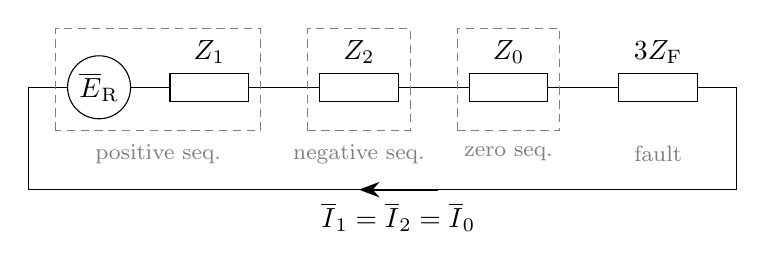
\begin{tikzpicture}[x=1cm,y=1cm]
% top rail
\draw (0,0) -- (0.5,0);
\draw (0.9,0) circle (0.4);
\node at (0.9,0) {$\pE{R}$};
\draw (1.3,0) -- (1.8,0);
\draw (1.8,-0.18) rectangle (2.8,0.18);
\node at (2.3,0.45) {$Z_{1}$};
\draw (2.8,0) -- (3.7,0);
\draw (3.7,-0.18) rectangle (4.7,0.18);
\node at (4.2,0.45) {$Z_{2}$};
\draw (4.7,0) -- (5.6,0);
\draw (5.6,-0.18) rectangle (6.6,0.18);
\node at (6.1,0.45) {$Z_{0}$};
\draw (6.6,0) -- (7.5,0);
\draw (7.5,-0.18) rectangle (8.5,0.18);
\node at (8.0,0.45) {$3Z_\mathrm{F}$};
\draw (8.5,0) -- (9.0,0);
% return rail
\draw (9.0,0) -- (9.0,-1.3) -- (0,-1.3) -- (0,0);
\draw[-{Stealth[length=2.6mm]},thick] (5.2,-1.3) -- (4.2,-1.3);
\node at (4.7,-1.65) {$\pI{1}=\pI{2}=\pI{0}$};
% group boxes
\draw[densely dashed,gray] (0.35,-0.55) rectangle (2.95,0.75);
\node[gray] at (1.65,-0.85) {\footnotesize positive seq.};
\draw[densely dashed,gray] (3.55,-0.55) rectangle (4.85,0.75);
\node[gray] at (4.2,-0.85) {\footnotesize negative seq.};
\draw[densely dashed,gray] (5.45,-0.55) rectangle (6.75,0.75);
\node[gray] at (6.1,-0.85) {\footnotesize zero seq.};
\node[gray] at (8.0,-0.85) {\footnotesize fault};
\end{tikzpicture}
\caption{Series connection of the sequence networks for a single
phase-to-earth fault on phase R through $Z_\mathrm{F}$.}
\label{fig:seqnet}
\end{figure}

\subsection{Phase-to-earth voltages at the fault}

With $Z_{2}=Z_{1}$ and a bolted fault ($Z_\mathrm{F}=0$), the sequence
voltages at the fault are $\overline{U}_{1}=\pE{R}(Z_{0}+Z_{1})/(Z_{0}+2Z_{1})$,
$\overline{U}_{2}=-\pE{R}\,Z_{1}/(Z_{0}+2Z_{1})$ and
$\overline{U}_{0}=-\pE{R}\,Z_{0}/(Z_{0}+2Z_{1})$. Transforming back to phase
quantities gives the compact result
\begin{equation}
\boxed{\;
\pU{R} = 0, \qquad
\pU{S} = \left(a^{2}-k\right)\pE{R}, \qquad
\pU{T} = \left(a-k\right)\pE{R}, \qquad
k \triangleq \frac{Z_{0}-Z_{1}}{Z_{0}+2Z_{1}} .
\;}
\label{eq:Vphase}
\end{equation}
The complex factor $k$ contains the entire influence of the earthing method.
Graphically, \eqref{eq:Vphase} states that the healthy-phase phasors keep
their pre-fault orientation and are shifted rigidly by $-k\pE{R}$, i.e.\ the
effective earth reference point moves by $k\pE{R}$ towards the faulted-phase
vertex of the voltage triangle. The zero-sequence voltage, which is what
residual-voltage relays measure, is
\begin{equation}
\overline{U}_{0} = \tfrac{1}{3}\left(\pU{R}+\pU{S}+\pU{T}\right)
 = -\frac{Z_{0}}{Z_{0}+2Z_{1}}\,\pE{R}.
\label{eq:V0}
\end{equation}

Two invariants are worth noting. First, $\pU{ST}=\pU{S}-\pU{T}=(a^{2}-a)\pE{R}$
is identical to its pre-fault value for any $k$: the line-to-line voltage
between the healthy phases never changes. Second, the line-to-line voltages
involving the faulted phase, $\pU{RS}$ and $\pU{RT}$, have magnitude
$|k-a^{2}|\,E$ and are reduced only when significant fault current flows
($k\to 0$); in an isolated network ($k\to 1$) the whole line-to-line triangle
is preserved.

\subsection{Earth fault factor}

The earth fault factor $k_\mathrm{e}$ (IEC~60071-1) is the ratio between the
highest healthy phase-to-earth voltage during the fault and the pre-fault
phase-to-earth voltage at the same location. From \eqref{eq:Vphase}, for real
$k$,
\begin{equation}
k_\mathrm{e} = \left|a^{2}-k\right| = \sqrt{k^{2}+k+1}.
\label{eq:ke}
\end{equation}
For purely inductive impedances with $m = X_{0}/X_{1}$, $k = (m-1)/(m+2)$.
Table~\ref{tab:ke} gives representative values. A system is called
\emph{effectively earthed} when $X_{0}/X_{1}\le 3$ and $R_{0}/X_{1}\le 1$,
which bounds $k_\mathrm{e}$ to about 1.4; insulation, surge arresters and
equipment withstand are coordinated on this basis.

\begin{table}[htb]
\centering
\caption{Earth fault factor versus zero-to-positive sequence reactance ratio
(purely inductive network, bolted fault, $Z_2=Z_1$).}
\label{tab:ke}
\begin{tabular}{ccc}
\toprule
$X_{0}/X_{1}$ & $k$ & $k_\mathrm{e}$ \\
\midrule
1 & 0 & 1.00 \\
2 & 0.25 & 1.15 \\
3 & 0.40 & 1.25 \\
5 & 0.57 & 1.38 \\
10 & 0.75 & 1.52 \\
$\to\infty$ & $\to 1$ & $\to\sqrt{3}\approx 1.73$ \\
\bottomrule
\end{tabular}
\end{table}

In an isolated-neutral network the zero-sequence impedance is capacitive,
$Z_{0}\simeq 1/(j\omega C_\mathrm{E})$ per phase with $C_\mathrm{E}$ the
phase-to-earth capacitance, so that
$k = (X_\mathrm{C0}+X_{1})/(X_\mathrm{C0}-2X_{1})$ is slightly \emph{greater}
than one and the healthy phases can exceed $\sqrt{3}\,E$ by a few percent even
in steady state. Larger overvoltages in isolated networks come from the
transient phenomena discussed in Section~\ref{sec:transients}.

\section{Behaviour by Earthing Method}
\label{sec:earthing}

\subsection{Isolated neutral}
\label{sec:isolated}

With the neutral isolated, the only zero-sequence path is the phase-to-earth
capacitance and $|Z_{0}|\gg|Z_{1}|$, hence $k\simeq 1$. The picture is the
classic one of Fig.~\ref{fig:isolated}: the line-to-line voltage triangle RST
is unchanged, and the earth reference point moves from the centroid N to the
faulted-phase vertex R. Consequently:
\begin{equation}
\pU{R}=0, \qquad
|\pU{S}| = |\pU{T}| = \sqrt{3}\,E, \qquad
\overline{U}_{0} = -\pE{R},
\end{equation}
with an angle of \ang{60} between $\pU{S}$ and $\pU{T}$ instead of the
pre-fault \ang{120}. The residual voltage reaches its maximum possible value,
$|3\overline{U}_{0}| = 3E$, which makes detection trivial, while the fault
current is only the capacitive current of the two healthy phases,
\begin{equation}
|\pI{\ph{F}}| \simeq 3\,\omega C_\mathrm{E}\,E
            = \sqrt{3}\,\omega C_\mathrm{E}\,U_\mathrm{n},
\end{equation}
typically a few amperes to a few tens of amperes in a medium-voltage cable
network. Loads and converters connected line-to-line are unaffected, and
operation can continue during the fault; the price is that the entire network
insulation must withstand line-to-line voltage to earth for the duration of
the fault, and that a second earth fault on another phase (cross-country
fault) short-circuits two phases through earth.

\subsection{Resonant earthing (Petersen coil)}

With an arc-suppression coil $L_\mathrm{P}$ between neutral and earth tuned to
the network capacitance, $3\omega^{2}L_\mathrm{P}C_\mathrm{E}\simeq 1$, the
inductive neutral current cancels the capacitive fault current, leaving only a
small resistive and harmonic residual. The steady-state voltage picture is the
same as in the isolated case ($k\simeq 1$, healthy phases at $\sqrt{3}\,E$,
full neutral displacement), but the near-zero current at the fault point
allows arc self-extinction in air-insulated networks and permits sustained
operation with the fault present. This is the standard practice in most
European medium-voltage networks, including the Italian ones, which migrated
from isolated to compensated neutral in the 2000s.

\subsection{Effective and solid earthing}

With the neutral solidly earthed or earthed through a low impedance,
$Z_{0}$ is comparable to $Z_{1}$, $k$ is small, and the fault becomes a true
short circuit: the faulted phase voltage collapses over a wide area, the
healthy phases rise moderately ($k_\mathrm{e}\le 1.4$ for effective earthing),
and the fault current is of the same order as the three-phase short-circuit
current. Fast selective tripping is mandatory. This is the usual arrangement
in transmission networks and in low-voltage TN systems. From the point of
view of connected equipment the event is a single-phase voltage dip with
moderate swell on the healthy phases, rather than a neutral displacement.

\section{Phasor Diagrams in the RST Plane}
\label{sec:diagrams}

All diagrams are drawn in a common frame with the earth potential G at the
origin, phase R pointing upwards, and voltages in per unit of $E$. Dashed grey
phasors are the pre-fault quantities, thick black phasors the quantities
during the fault.

Fig.~\ref{fig:healthy} shows the balanced pre-fault condition: the star of
$\pE{R}$, $\pE{S}$, $\pE{T}$ with the neutral point N coincident with earth G,
and the line-to-line triangle RST.

\begin{figure}[htb]
\centering
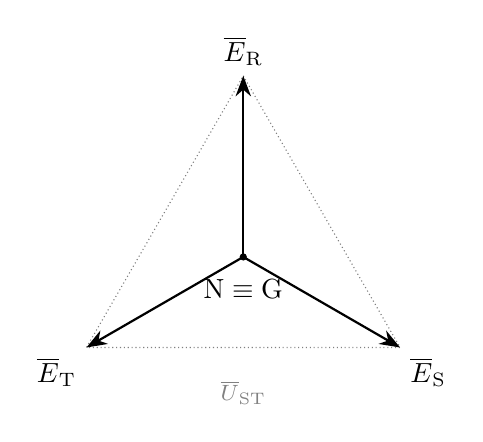
\begin{tikzpicture}[scale=2.3]
\coordinate (O) at (0,0);
\coordinate (R) at (0,1);
\coordinate (S) at (0.866,-0.5);
\coordinate (T) at (-0.866,-0.5);
\draw[construction] (R) -- (S) -- (T) -- cycle;
\draw[phasor] (O) -- (R) node[above] {$\pE{R}$};
\draw[phasor] (O) -- (S) node[below right] {$\pE{S}$};
\draw[phasor] (O) -- (T) node[below left] {$\pE{T}$};
\fill (O) circle (0.02);
\node[below] at (0,-0.07) {$\mathrm{N}\equiv\mathrm{G}$};
\node[gray] at (0,-0.75) {\footnotesize $\pU{ST}$};
\end{tikzpicture}
\caption{Balanced pre-fault condition: neutral point N at earth potential,
symmetric star of phase-to-earth voltages, line-to-line triangle RST (dotted).}
\label{fig:healthy}
\end{figure}

Fig.~\ref{fig:isolated} shows the bolted fault on phase R in an
isolated-neutral (or resonant-earthed) network, $k=1$. The triangle RST is
rigid and simply translates by $-\pE{R}$: vertex R lands on the earth point G,
the neutral N moves to $-\pE{R}$, and the phase-to-earth voltages of the
healthy phases become the line-to-line phasors $\pU{S}'=\pU{SR}$ and
$\pU{T}'=\pU{TR}$, of magnitude $\sqrt{3}\,E$ and \ang{60} apart.

\begin{figure}[htb]
\centering
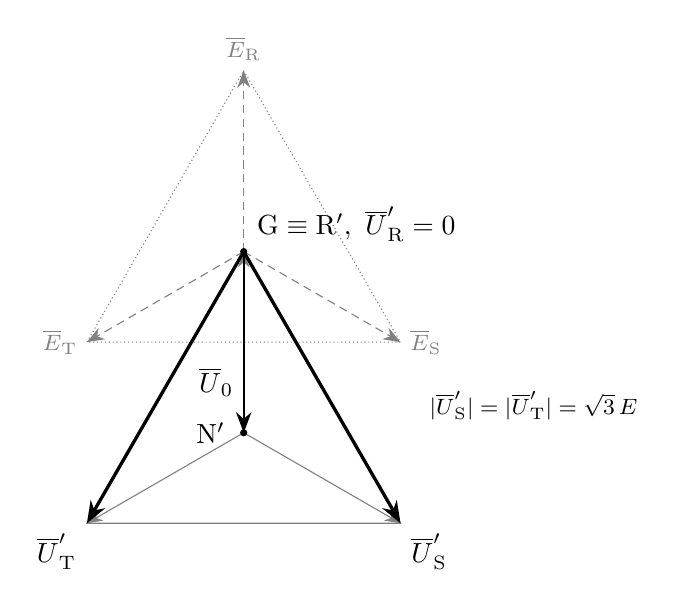
\begin{tikzpicture}[scale=2.3]
\coordinate (O) at (0,0);
\coordinate (R) at (0,1);
\coordinate (S) at (0.866,-0.5);
\coordinate (T) at (-0.866,-0.5);
\coordinate (Np) at (0,-1);
\coordinate (Rp) at (0,0);
\coordinate (Sp) at (0.866,-1.5);
\coordinate (Tp) at (-0.866,-1.5);
% pre-fault
\draw[pre] (O) -- (R) node[above] {\footnotesize $\pE{R}$};
\draw[pre] (O) -- (S) node[right] {\footnotesize $\pE{S}$};
\draw[pre] (O) -- (T) node[left] {\footnotesize $\pE{T}$};
\draw[construction] (R) -- (S) -- (T) -- cycle;
% displaced triangle and EMFs from displaced neutral
\draw[faulttriangle] (Rp) -- (Sp) -- (Tp) -- cycle;
\draw[emf] (Np) -- (Rp);
\draw[emf] (Np) -- (Sp);
\draw[emf] (Np) -- (Tp);
% fault phasors from earth
\draw[faultphasor] (O) -- (Sp) node[below right] {$\pU{S}'$};
\draw[faultphasor] (O) -- (Tp) node[below left] {$\pU{T}'$};
\draw[phasor] (O) -- (Np) node[pos=0.72,left] {$\overline{U}_{0}$};
\fill (O) circle (0.02);
\node[above right] at (0.02,0.0) {$\mathrm{G}\equiv\mathrm{R}',\ \pU{R}'=0$};
\fill (Np) circle (0.02);
\node[left] at (-0.05,-1) {$\mathrm{N}'$};
\node at (1.6,-0.85) {\footnotesize $|\pU{S}'|=|\pU{T}'|=\sqrt{3}\,E$};
\end{tikzpicture}
\caption{Bolted fault on phase R, isolated or resonant-earthed neutral
($k=1$). The rigid voltage triangle translates so that vertex R coincides
with earth: the neutral displaces fully
($\overline{U}_{0}=-\pE{R}$) and the healthy phases rise to line-to-line
magnitude, \ang{60} apart.}
\label{fig:isolated}
\end{figure}

Fig.~\ref{fig:effective} shows the same fault in an effectively earthed
network with $X_{0}/X_{1}=3$, i.e.\ $k=0.4$. The healthy-phase phasors shift
by $-0.4\,\pE{R}$, giving $k_\mathrm{e}=1.25$. The triangle is no longer
rigid: R collapses onto G, so $\pU{RS}$ and $\pU{RT}$ shrink from
$\sqrt{3}\,E$ to $1.25\,E$, while the base $\pU{ST}$ is unchanged. The
zero-sequence voltage is $\overline{U}_{0}=-0.6\,\pE{R}$.

\begin{figure}[htb]
\centering
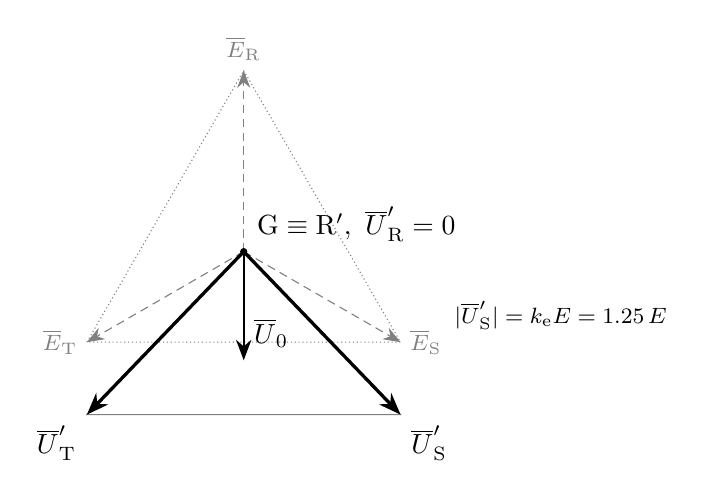
\begin{tikzpicture}[scale=2.3]
\coordinate (O) at (0,0);
\coordinate (R) at (0,1);
\coordinate (S) at (0.866,-0.5);
\coordinate (T) at (-0.866,-0.5);
\coordinate (Sp) at (0.866,-0.9);
\coordinate (Tp) at (-0.866,-0.9);
\coordinate (V0) at (0,-0.6);
% pre-fault
\draw[pre] (O) -- (R) node[above] {\footnotesize $\pE{R}$};
\draw[pre] (O) -- (S) node[right] {\footnotesize $\pE{S}$};
\draw[pre] (O) -- (T) node[left] {\footnotesize $\pE{T}$};
\draw[construction] (R) -- (S) -- (T) -- cycle;
% distorted triangle during fault
\draw[faulttriangle] (O) -- (Sp) -- (Tp) -- cycle;
% fault phasors
\draw[faultphasor] (O) -- (Sp) node[below right] {$\pU{S}'$};
\draw[faultphasor] (O) -- (Tp) node[below left] {$\pU{T}'$};
\draw[phasor] (O) -- (V0) node[pos=0.75,right] {$\overline{U}_{0}$};
\fill (O) circle (0.02);
\node[above right] at (0.02,0.0) {$\mathrm{G}\equiv\mathrm{R}',\ \pU{R}'=0$};
\node at (1.75,-0.35) {\footnotesize $|\pU{S}'|=k_\mathrm{e}E=1.25\,E$};
\end{tikzpicture}
\caption{Bolted fault on phase R, effectively earthed network with
$X_{0}/X_{1}=3$ ($k=0.4$). The healthy phases rise only to
$k_\mathrm{e}=1.25$, the triangle distorts ($\pU{RS}$, $\pU{RT}$ reduced,
$\pU{ST}$ unchanged) and the neutral displacement is partial,
$\overline{U}_{0}=-0.6\,\pE{R}$.}
\label{fig:effective}
\end{figure}

\section{Fault Resistance and Neutral Displacement Locus}
\label{sec:locus}

Real earth faults are rarely bolted: tree contact, surface arcing and cable
sheath faults present resistances from a few ohms to tens of
\si{\kilo\ohm}. In an isolated network, neglecting the series impedance
$Z_{1}$ against the capacitive $Z_{0}$, the neutral displacement for a fault
through $R_\mathrm{F}$ is
\begin{equation}
\overline{U}_\mathrm{N}
 = -\,\frac{\pE{R}}{1+j\,3\omega C_\mathrm{E} R_\mathrm{F}} .
\label{eq:locus}
\end{equation}
As $R_\mathrm{F}$ sweeps from $0$ to $\infty$, \eqref{eq:locus} is a bilinear
map of a real parameter and $\overline{U}_\mathrm{N}$ travels along a
semicircle of diameter $E$ between $-\pE{R}$ and the origin
(Fig.~\ref{fig:locus}). The practical consequence for protection is that the
residual voltage $|3\overline{U}_{0}|$ decreases monotonically with
$R_\mathrm{F}$: a relay set at, say, $0.3\,E$ residual (10\,\% of $3E$)
detects faults only up to
$R_\mathrm{F} \simeq \sqrt{10}/(\omega\,3 C_\mathrm{E})$, and
high-resistance faults require sensitive directional (wattmetric) methods
based on $\overline{U}_{0}$ and $\pI{0}$ together.

\begin{figure}[htb]
\centering
\begin{tikzpicture}[scale=2.3]
\coordinate (O) at (0,0);
\coordinate (R) at (0,1);
\coordinate (S) at (0.866,-0.5);
\coordinate (T) at (-0.866,-0.5);
\coordinate (Nb) at (0,-1);
\coordinate (M) at (-0.5,-0.5);
% pre-fault star (light)
\draw[pre] (O) -- (R) node[above] {\footnotesize $\pE{R}$};
% locus
\draw[thick] (Nb) arc[start angle=-90, end angle=-270, radius=0.5];
\draw[-{Stealth[length=2.4mm]},thick] (Nb) arc[start angle=-90, end angle=-160, radius=0.5];
% sample phasor
\draw[faultphasor] (O) -- (M) node[pos=0.55,above left] {$\overline{U}_\mathrm{N}$};
\fill (Nb) circle (0.02);
\node[right] at (0.05,-1) {\footnotesize $R_\mathrm{F}=0:\ \overline{U}_\mathrm{N}=-\pE{R}$};
\fill (O) circle (0.02);
\node[below right] at (0.05,-0.02) {\footnotesize $R_\mathrm{F}\to\infty$};
\fill (M) circle (0.02);
\node[left] at (-0.55,-0.5) {\footnotesize $3\omega C_\mathrm{E}R_\mathrm{F}=1$};
\end{tikzpicture}
\caption{Locus of the neutral displacement $\overline{U}_\mathrm{N}$ in an
isolated-neutral network as the fault resistance $R_\mathrm{F}$ varies from
$0$ (full displacement) to $\infty$ (no displacement). The arrow indicates
increasing $R_\mathrm{F}$.}
\label{fig:locus}
\end{figure}

\section{Transient Phenomena}
\label{sec:transients}

The phasor picture describes the steady state reached a few cycles after
fault inception. The inception itself is accompanied by a high-frequency
transient in which the healthy-phase capacitances recharge from phase to
line-to-line voltage through the network series inductance, producing an
oscillatory overshoot on the healthy phases well above $\sqrt{3}\,E$. In
isolated networks, an unstable arc that extinguishes and restrikes near the
current zeros (arcing ground fault) can pump this mechanism repeatedly and
build phase-to-earth overvoltages historically quoted up to about
$3\,$--$\,3.5$ per unit; this, together with the cross-country fault risk of
Section~\ref{sec:isolated}, is the main argument for resonant earthing or for
adding a neutral resistor. In effectively earthed networks the transient is a
conventional short-circuit transient with DC offset in the fault current, and
temporary overvoltages remain bounded by $k_\mathrm{e}$.

\section{Propagation Through a Dy11 Transformer}
\label{sec:dy11}

\subsection{Sequence transformation rules}

A transformer of vector group Dy11 (delta primary, wye secondary, clock
number 11) transfers the sequence voltages between its terminals as, in per
unit,
\begin{equation}
\overline{U}_{1}' = e^{+j30^{\circ}}\,\overline{U}_{1}, \qquad
\overline{U}_{2}' = e^{-j30^{\circ}}\,\overline{U}_{2}, \qquad
\overline{U}_{0}' = 0 :
\label{eq:dy11rules}
\end{equation}
the positive sequence is rotated by $+\ang{30}$ (secondary leads), the
negative sequence by $-\ang{30}$, and the zero sequence is not transferred at
all. The delta winding is excited only by the line-to-line voltages of the
primary network, so the neutral displacement of Section~\ref{sec:earthing}
never reaches the secondary: the potential of the secondary star point is
fixed by its own earthing, independently of the primary fault. Whether the
secondary neutral is earthed (Dyn11) or not is irrelevant for a primary-side
fault, since no secondary zero sequence is excited.

\subsection{Secondary voltages for a primary phase-to-earth fault}

Applying \eqref{eq:dy11rules} to the sequence voltages of
Section~\ref{sec:seq}, with secondary phases labelled r, s, t, gives for the
bolted fault on primary phase R (with $Z_{2}=Z_{1}$):
\begin{equation}
\pU{s}' = a^{2}e^{+j30^{\circ}}\overline{U}_{1}
        + a\,e^{-j30^{\circ}}\overline{U}_{2}
        = -j\,\pE{R},
\label{eq:dy11spared}
\end{equation}
i.e.\ one secondary phase retains \emph{exactly} its pre-fault value --- in
magnitude and in phase --- for every earthing method and even for a resistive
fault, because $a^{2}e^{+j30^{\circ}} = -j$ and $a\,e^{-j30^{\circ}} = +j$
cancel the equal series drops of the positive and negative sequence. The
other two phases dip symmetrically:
\begin{equation}
|\pU{r}'| = |\pU{t}'| = \frac{\sqrt{3+(1+2k)^{2}}}{2\sqrt{3}}\,E,
\qquad
\Delta\varphi = \arctan\!\frac{\sqrt{3}}{1+2k} - 30^{\circ},
\label{eq:dy11depth}
\end{equation}
with $\pU{r}'$ advanced and $\pU{t}'$ retarded by $\Delta\varphi$, so that the
two phasors close towards each other. Numerically: for $k=1$ (isolated or
resonant primary neutral) the secondary is completely unaffected, consistent
with the rigid line-to-line triangle of Fig.~\ref{fig:isolated}; for $k=0.4$
($X_{0}/X_{1}=3$) the two phases drop to $0.72\,E$ with
$\Delta\varphi\approx\ang{14}$; for the deepest case $k=0$ ($Z_{0}=Z_{1}$)
they drop to $E/\sqrt{3}\approx 0.58\,E$ with $\Delta\varphi=\ang{30}$
(Fig.~\ref{fig:dy11}). In the Bollen classification the transformer converts
the type~B dip (single phase to earth, with zero sequence) into a type~C dip
(two phases reduced and closed towards each other, one phase intact). Two
practical consequences follow: downstream of a Dy11 no phase-to-earth voltage
ever drops below $1/\sqrt{3}$ of nominal for a single phase-to-earth fault,
and one phase is always spared --- which phase depends on the faulted primary
phase and on the clock number. A fault impedance $Z_\mathrm{F}>0$ only makes
the dip shallower, while \eqref{eq:dy11spared} continues to hold exactly.

\begin{figure}[htb]
\centering
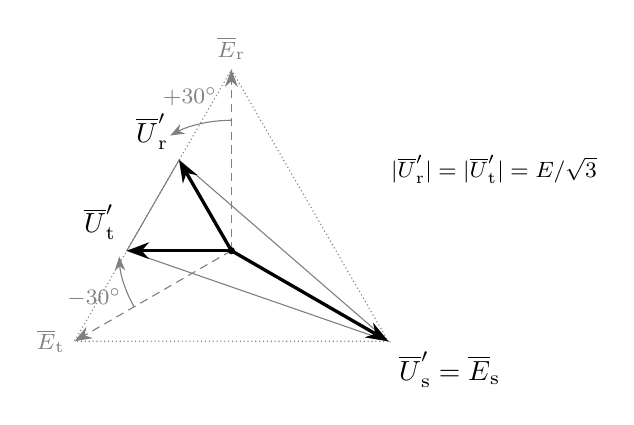
\begin{tikzpicture}[scale=2.3]
\coordinate (O) at (0,0);
\coordinate (r) at (0,1);
\coordinate (s) at (0.866,-0.5);
\coordinate (t) at (-0.866,-0.5);
\coordinate (rp) at (-0.289,0.5);
\coordinate (tp) at (-0.577,0);
% pre-fault
\draw[pre] (O) -- (r) node[above] {\footnotesize $\pE{r}$};
\draw[pre] (O) -- (s);
\draw[pre] (O) -- (t) node[left] {\footnotesize $\pE{t}$};
\draw[construction] (r) -- (s) -- (t) -- cycle;
% during-fault triangle
\draw[faulttriangle] (rp) -- (s) -- (tp) -- cycle;
% fault phasors
\draw[faultphasor] (O) -- (rp) node[above left] {$\pU{r}'$};
\draw[faultphasor] (O) -- (tp) node[above left] {$\pU{t}'$};
\draw[faultphasor] (O) -- (s) node[below right] {$\pU{s}'=\pE{s}$};
% phase-jump arcs
\draw[-{Stealth[length=1.8mm]},thin,gray]
  (90:0.72) arc[start angle=90, end angle=118, radius=0.72];
\node[gray] at (105:0.88) {\footnotesize $+\ang{30}$};
\draw[-{Stealth[length=1.8mm]},thin,gray]
  (210:0.62) arc[start angle=210, end angle=183, radius=0.62];
\node[gray] at (199:0.80) {\footnotesize $-\ang{30}$};
\fill (O) circle (0.02);
\node at (1.45,0.45) {\footnotesize $|\pU{r}'|=|\pU{t}'|=E/\sqrt{3}$};
\end{tikzpicture}
\caption{Secondary phase-to-earth voltages downstream of a Dy11 transformer
for a bolted phase-to-earth fault on primary phase R, drawn for $k=0$
($Z_{0}=Z_{1}$) in the secondary frame (the fixed \ang{30} group displacement
is omitted for clarity). Phase s is unaffected for every $k$; phases r and t
drop to $E/\sqrt{3}$ and jump \ang{30} towards each other (dip type~C). For
$k\to 1$ all three secondary voltages are unchanged.}
\label{fig:dy11}
\end{figure}

\subsection{Secondary-side earth fault seen from the primary}

The blocking works in both directions. For an earth fault on the
earthed-wye secondary side, the zero-sequence current circulates inside the
delta winding and never appears in the primary lines: with sequence current
$\pI{}$ in the fault loop, the secondary line currents are $(3\pI{},\,0,\,0)$
while the primary line currents are $(\sqrt{3}\pI{},\,\sqrt{3}\pI{},\,0)$ in
per unit --- two primary lines carry equal current and the residual
(zero-sequence) current on the primary side is identically zero. Seen from
the primary network the fault therefore looks like a phase-to-phase event,
and primary residual-current earth-fault protection is structurally blind to
it: secondary earth faults must be cleared by secondary-side protection or by
a relay in the transformer star-point connection.

\section{Impact on Grid-Connected Converters}
\label{sec:converters}

For grid-connected converters the relevant points are these. A three-wire
converter without earthed midpoint provides no zero-sequence current path, so
the fault affects it only through the line-to-line voltages and through the
common-mode potential of the whole DC link, which follows the neutral
displacement and stresses the phase-to-earth insulation, EMI filter Y
capacitors and any earth-leakage monitoring. Synchronisation should be
performed on the positive-sequence component (e.g.\ DDSRF- or DSOGI-based
PLL): a per-phase or zero-sequence-sensitive PLL sees the full neutral
displacement and can lose lock even though the line-to-line voltages are
intact. In effectively earthed networks the fault appears as an asymmetric
dip: the negative-sequence voltage drives double-frequency power and DC-link
ripple, and ride-through with controlled positive- and negative-sequence
current injection is required by most grid codes. Finally, converters with an
earthed DC midpoint or four-wire output do provide a zero-sequence path and
must limit the resulting current actively during the neutral displacement.

\section{Summary}

The single phase-to-earth fault moves the network voltages in a way that is
entirely governed by the ratio $Z_{0}/Z_{1}$, condensed in the factor
$k=(Z_{0}-Z_{1})/(Z_{0}+2Z_{1})$: the faulted phase-to-earth voltage
collapses, the healthy ones become $(a^{2}-k)\pE{R}$ and $(a-k)\pE{R}$, and a
zero-sequence voltage $-\pE{R}Z_{0}/(Z_{0}+2Z_{1})$ appears. In isolated and
resonant-earthed networks ($k\simeq 1$) the line-to-line triangle is rigid,
the earth point moves to the faulted vertex and the healthy phases reach
$\sqrt{3}\,E$; in effectively earthed networks ($k$ small) the event is a
single-phase short circuit with moderate rise of the healthy phases,
$k_\mathrm{e}\le 1.4$. The line-to-line voltage between the healthy phases is
invariant in all cases, which is why line-to-line connected equipment, and
converters synchronised on the positive sequence, ride through the
disturbance naturally. Downstream of a Dy11 transformer the fault loses its
zero sequence entirely: one secondary phase is exactly unaffected and the
other two drop at most to $E/\sqrt{3}$ with $\pm\ang{30}$ phase jumps towards
each other (type~C dip), while a secondary-side earth fault produces no
residual current on the primary lines.

\begin{thebibliography}{9}

\bibitem{anderson}
P.~M. Anderson, \emph{Analysis of Faulted Power Systems}. Piscataway, NJ:
IEEE Press, 1995.

\bibitem{blackburn}
J.~L. Blackburn, \emph{Symmetrical Components for Power Systems Engineering}.
New York: Marcel Dekker, 1993.

\bibitem{willheim}
R.~Willheim and M.~Waters, \emph{Neutral Grounding in High-Voltage
Transmission}. New York: Elsevier, 1956.

\bibitem{iec60071}
\emph{Insulation Co-ordination -- Part 1: Definitions, Principles and Rules},
IEC Standard 60071-1, 2019.

\bibitem{ieee-c6292}
\emph{IEEE Guide for the Application of Neutral Grounding in Electrical
Utility Systems -- Part I: Introduction}, IEEE Standard C62.92.1, 2016.

\bibitem{bollen}
M.~H.~J. Bollen, \emph{Understanding Power Quality Problems: Voltage Sags and
Interruptions}. Piscataway, NJ: IEEE Press, 2000.

\end{thebibliography}

\end{document}
